\question \textbf{DP with score matrix}
  
Use the score matrix below with gap penalty g =1 and answer the following questions.

\begin{figure}[h]
  \centering
      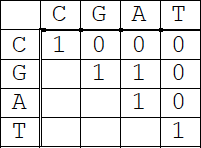
\includegraphics[width=0.2 \textwidth]{fig03/simple_score_matrix.png}
\end{figure}

\begin{parts}

%% (a)
  \part	Calculate the alignment score.

\begin{itemize}
\item Alignment 1
\begin{verbatim}
    q: ATGCT
    d: CA--T \end{verbatim}
    
\begin{solution}[0.35 in]
  1
\end{solution}
  
\item Alignment 2
\begin{verbatim}
    q: CAGCT
    d: C-A-T \end{verbatim}
  
\begin{solution}[0.35 in]
  1
\end{solution}

\end{itemize}

%% (b)
\part Use the simple scorning scheme and fill the empty cells with appropriate scores.

\begin{itemize}
\item Table A
\begin{figure}[h]
  \centering
      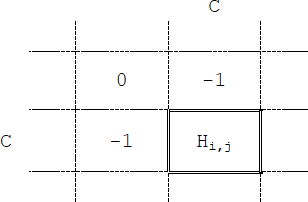
\includegraphics[width=0.25 \textwidth]{fig03/cell_update_score_matrix_1.png}
\end{figure}

\begin{solution}[0.75 in]
1
\end{solution}

\item Table B
\begin{figure}[!h]
  \centering
      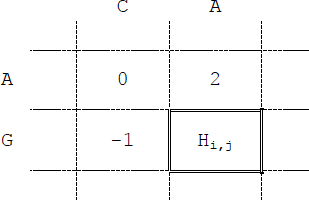
\includegraphics[width=0.25 \textwidth]{fig03/cell_update_score_matrix_2.png}
\end{figure}

\begin{solution}[0.75 in]
1
\end{solution}

\end{itemize}

\pagebreak

%% (c)
\part Fill the empty cells with appropriate scores in the DP table. What is the optimal alignment score?

\begin{figure}[h]
  \centering
      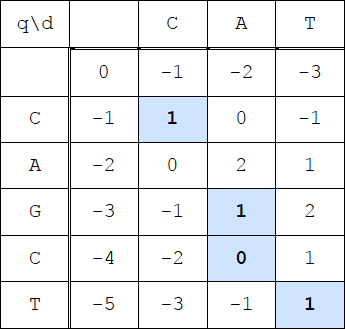
\includegraphics[width=0.35 \textwidth]{fig03/dp_with_score_matrix_solution.png}
\end{figure}

\begin{solution}[0.75 in]
1
\end{solution}

%% (d)
\part There are two different alignments that give the same optimal score in the solution above. Specify both of them.

\begin{solution}[1.75 in]
\begin{verbatim}
  q: CAGCT
  d: CA--T
  
  q: CAGCT
  d: C-A-T
\end{verbatim}
\end{solution}

\end{parts}

\pagebreak
